\documentclass[a4paper, 11pt]{article}
\usepackage{comment} % enables the use of multi-line comments (\ifx \fi) 
\usepackage{fullpage} % changes the margin

\usepackage{tabu} % for nice arrays	
% For confusion matrix %
\usepackage{array}
\usepackage{multirow}

\newcommand\MyBox[2]{
  \fbox{\lower0.75cm
     \vbox to 1.7cm{\vfil
      \hbox to 1.7cm{\hfil\parbox{1.4cm}{#1\\#2}\hfil}
      \vfil}%
   }%
}
%%%%%%%%%%%%%%%%%%%%%%%%%
\usepackage{graphicx} % For img insert
\newcommand{\ts}{\textsuperscript} %For numering 1st 2nd
%% Greek Format %%
%\usepackage[cm-default]{fontspec}
%\setromanfont{FreeSerif}
%\setsansfont{FreeSans}
%\setmonofont{FreeMono}
\usepackage{xltxtra}
\usepackage{xgreek}
\setmainfont[Mapping=tex-text]{GFS Didot}
%%%%%%%%%%%%%%%%%%

\begin{document}
%Header-Make sure you update this information!!!!
\noindent
\large\textbf{Αναφορά Διπλωματικής 1} \hfill \textbf{Αθανάσιος Μητσέλος} \\
\normalsize ΣΗΜΜΥ \hfill Ημερομηνία Ανάθεσης: 6/12/17  \\
ΕΜΠ\hfill Τρέχουσα Ημερομηνία: 1/04/17 \\


\section*{Eξαγωγή Δεδομένων και Προετοιμασία}
Τα υπό έρευνα δεδομένα περιλαμβάνουν μετρήσεις καταναλώσεων έξυπνων μετρητών από απλούς καταναλωτές και μικρο-μεσαίες επιχειρήσεις. Συνολικά πρόκειται για δεδομένα περίπου 5500 έξυπνων μετρητών με καταγραφή της κατανάλωσης κάθε 30 λεπτά και με διάρκεια σχεδόν 2 έτη, από το καλοκαίρι του 2009 μέχρι το τέλος του 2010. Πρόκειται για αντιπροσωπευτικά δείγματα που συλλέχθηκαν ανώνυμα από το "Irish Social Science Date Archive Center" \cite{NeuralNet}. \\
\begin{enumerate}
\item{Επιλογή Δεδομένων}\\
Σε πρώτη φάση, χρειάστηκε να βρεθούν καταναλωτές με συνεχή αποτελέσματα για ένα συγκεκριμένο χρονικό διάστημα, ώστε να δημιουργηθεί μια πλήρης χρονοσειρά για κάθε καταναλωτή. Θέτοντας το χρονικό αυτό διάστημα στο ένα έτος, δημιουργούμε ένα νέο πίνακα μετρήσεων που περιλαμβάνει 
μόνο καταναλωτές με αδιάλειπτες μετρήσεις για ένα έτος από την 1\ts{η} Ιανουαρίου μέχρι και την 31\ts{η} Δεκέμβριο του 2010. Με αυτόν τον τρόπο δημιουργήθηκε ένα πλήθος $K$ πινάκων που αντιστοιχεί στο πλήθος των καταναλωτών διάστασης ($NxM$) με $N$ να είναι μια υποδιαίρεση του έτους όπως ημέρες (365) και $M$ να είναι μια υποδιαίρεση του $N$ όπως ώρες (24). \\
\item Επιλογή Χαρακτηριστικών\\
Σε δεύτερη φάση, δημιουργήθηκε η ανάγκη για εξαγωγή χαρακτηριστικών, ώστε να μειωθούν οι διαστάσεις των πινάκων και να επιταχυνθεί η διαδικασία. Παράλληλα, παρέχει ένα επίπεδο αποπροσωποποίησης δημιουργώντας ένα αποτύπωμα της καταναλωτικής συνήθειας.\cite{giwrgis}. Μετρώντας τα αθροίσματα, τα ελάχιστα, τα μέγιστα και τους μέσους όρους των καθημερινών καταναλώσεων δημιουργείται ένας βασικός κορμός χαρακτηριστικών για κάθε καταναλωτή που μπορεί εύκολα να επεκταθεί και σε άλλα γραμμικά και μη εξαρτώμενα χαρακτηριστικά.
\begin{itemize}
\item \textit{Μέγιστο και ώρα μεγίστου}
\item \textit{Ελάχιστο και ώρα ελαχίστου}
\item \textit{Άθροισμα κατανάλωσης ανά ημέρα}
\item \textit{Μέσος όρος, διακύμανση και τυπική απόκλιση ανά ημέρα}
\item \textit{Παράγοντας φορτίου, ελάχιστο προς μέση τιμή, ελάχιστο προς μέγιστο}
\item \textit{Επίδραση βραδινής κατανάλωσης}
\item \textit{Λοξότητα και Κύρτωση}
\end{itemize}
\end{enumerate}

\section*{Προσομοίωση απάτης}
Δεδομένου ότι οι μετρήσεις που συλλέχθηκαν ήταν από αξιόπιστους καταναλωτές θα πρέπει να μοντελοποιηθεί η συμπεριφορά με μη τεχνικές απώλειες. Έτσι, μοντελοποιήθηκαν 4 συμπεριφορές που καθεμία εισάγει έναν διαφορετικό παράγοντα \cite{patterns}. Για τις 3 πρώτους τύπους απωλειών εισάγεται μια τυχαία μέρα που ο καταναλωτής εγκαθιστά σύστημα αλλοίωσης των πραγματικών μετρήσεων. Παράλληλα, επιλέγεται η ένταση της κλοπής από μία κατανομή βήτα $Β(6,3)$. Η συνάρτηση πυκνότητας πιθανότητας για μια κατανομή $B(\alpha,\beta)$:\\
$f(x|\alpha, \beta)=\frac{x^{\alpha-1} \cdotp (1-x)^{\beta-1}}{\int_0^1 u^{\alpha-1} \cdotp (1-u)^{\beta-1}du}$
$=\frac{\Gamma(\alpha+\beta)}{\Gamma(\alpha) \cdotp \Gamma(\alpha)}x^{\alpha-1} \cdotp (1-x)^{\beta-1}$
$=\frac{1}{B(\alpha,\beta)}x^{\alpha-1} \cdotp (1-x)^{\beta-1}$
\begin{enumerate}

\item \textit{Απώλειες Τύπου 1} Μοντελοποιεί τον καταναλωτή που θα χρησιμοποιεί αδιάκοπα και μόνιμα το σύστημα αλλοίωσης μετρήσεων με τον ίδια ένταση.\\
\begin{figure}[ht!]
\centering
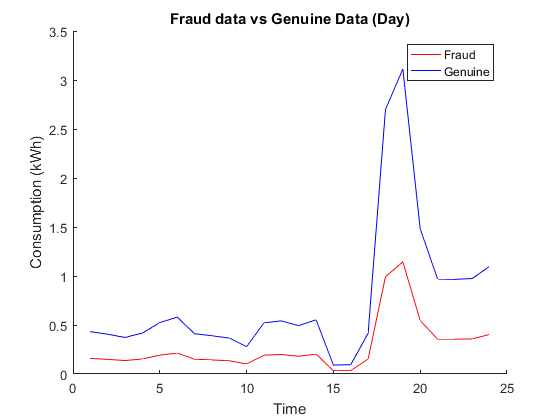
\includegraphics[width=110mm, height=70mm]{../../plots/type1.png}
\caption{Απώλειες Τύπου 1 \label{type1}}
\end{figure}

\item \textit{Απώλειες Τύπου 2} Μοντελοποιεί τον καταναλωτή που θα χρησιμοποιεί τυχαίες μέρες και για τυχαία διάρκεια μέσα στη μέρα σύστημα που αλλοιώνει τη μέτρηση με διαφορετική ένταση ανά ημέρα.\\
\begin{figure}[ht!]
\centering
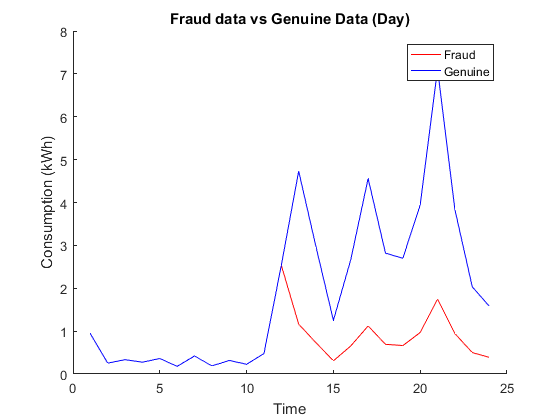
\includegraphics[width=110mm, height=70mm]{../../plots/type2_1.png}
\caption{Ημερήσια Απώλειες Τύπου 2\label{type2}}
\end{figure}

\newpage

\item \textit{Απώλειες Τύπου 3} Μοντελοποιεί τον καταναλωτή που θα χρησιμοποιεί τυχαίες μέρες και για τυχαία διάρκεια μέσα στη μέρα σύστημα που αλλοιώνει τη μέτρηση με διαφορετική ένταση ανά ώρα για κάθε διάρκεια.\\
\begin{figure}[ht!]
\centering
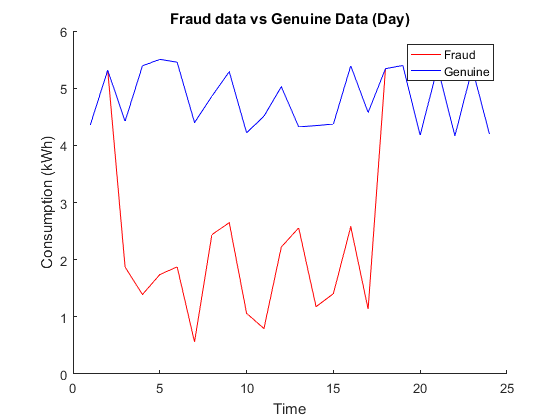
\includegraphics[width=110mm, height=70mm]{../../plots/type3.png}
\caption{Ημερήσια Απώλειες Τύπου 3 \label{type3}}
\end{figure}

\item \textit{Απώλειες Τύπου 4} Μοντελοποιεί τον καταναλωτή που εκτεμεταλλεύεται την κυμαινόμενη χρέωση και αλλοιώνει τις τιμές του κατά τέτοιο τρόπο ώστε η μεγάλη κατανάλωση να μεταφέρεται τις ώρες μειωμένης χρέωσης. \\
\begin{figure}[ht!]
\centering
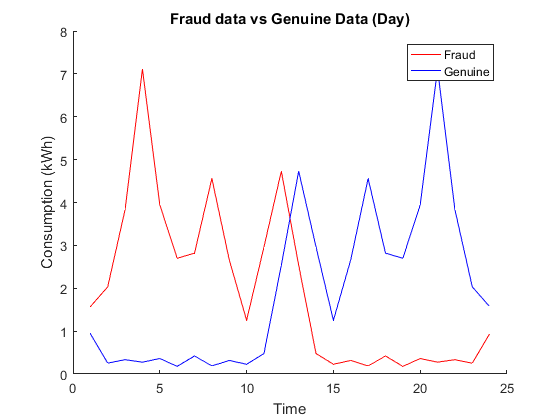
\includegraphics[width=110mm, height=70mm]{../../plots/type4.png}
\caption{Ημερήσια Απώλεια Τύπου 4 \label{type4}}
\end{figure}

\end{enumerate}
\newpage
\section*{Δεδομένα Εισόδου SVM}
Μία παράμετρος που έχει μεγάλη σημασία για τα αποτελέσματα του SVM, αλλά και για την ρεαλιστι-κότητα της προσομοίωσης είναι το ποσοστό FR (Fraud Rate)των καταναλωτών που αλλοιώνουν τις μετρήσεις τους. Αφού λοιπόν οργανωθούν οι ετήσιοι πίνακες κατανάλωσης στις υποδιαιρέσεις χρόνου με τις αντίστοιχες τιμές κατανάλωσης, εισάγονται στα δεδομένα οι μη τεχνικές απώλειες με σεβασμό στο FR. Μπορεί να χρησιμοποιηθεί οποιοσδήποτε τύπος
απωλειών, αλλά και συνδυασμός τους για ακόμα πιο αληθοφανή δεδομένα. Με αυτόν τον τρόπο εισάγεται αρκετή τυχαιότητα (Figure \ref{type3}), ώστε να ελαχιστοποιείται όσο γίνεται η απόκλιση από τις πραγματικές συνθήκες.\\
Η τελική μορφή των δεδομένων έρχεται μετά την εξαγωγή των χαρακτηριστικών από τα νοθευμένα δεδομένα και την κανονικοποίησή τους στο εύρος [0,1]. Το κύριο πλεονέκτημα της κανονικοποίησης είναι η αποφυγή της επιβολής των τιμών με μεγάλο αριθμητική εύρος στις τιμές με μικρότερο \cite{guide}. Τέλος, χρησιμοποιήθηκαν οι ίδιοι παράμετροι για την κανονικοποίηση των δεδομένων της εκπαίδευσης και της δοκιμής.

\section*{Επιλογή Παραμέτρων SVM}
Χρησιμοποιήθηκαν 3 διαφορετικοί τρόποι επιλογής παραμέτρων για τις παραμέτρους του SVM. Επιλέχθηκε ο "RBF Kernel", επειδή το πλήθος των χαρακτηριστικών $M$ είναι πολύ μικρότερο από το πλήθος των παραδειγμάτων $N$ δημιουργώντας ανάγκη να αποτυπωθούν τα δεδομένα σε μεγαλύτερη διάσταση \cite{guide} με έναν μη γραμμικό "Kernel". Ο τελευταίος περιγράφεται από δύο κυρίως παραμέτρους. Η μια είναι η μέση τιμή $C$, ενώ η άλλη είναι η γάμμα $\gamma$ που οποιαδήποτε και αν είναι πολύ μεγάλη θα έχουμε έναν πολύ ευαίσθητο ταξινομητή (overfitting) σε οποιαδήποτε νέα δεδομένα, πράγμα που δημιουργεί πρόβλημα στις δυνατότητες γενίκευσης, ενώ αν η τιμή είναι πολύ μικρή θα έχουμε έναν αλγόριθμο που θα δυσκολεύεται να ξεχωρίσει νέα δεδομένα λόγω της γενίκευσης που έχει επιβληθεί (underfitting).
\begin{center}
$K(X,X')=exp(-\frac{\|X-X'\|^2}{2\sigma^2})=exp(-\gamma\|X-X'\|^2)$
\end{center}

\begin{enumerate}
\item \textit{Γρήγορη αναζήτηση} Το μοναδικό πλεονέκτημα αυτής της αναζήτησης είναι η ταχύτητά της, αφού δεν δοκιμάζονται όλα τα δεδομένα και για εκπαίδευση και για δοκιμή και δεν συλλέγονται δεδομένα από όλους τους καταναλωτές για την εκπαίδευση και τη δοκιμή. Δεν είναι λοιπόν απίθανο τα δεδομένα που θα εξαχθούν να είναι αντιπροσωπευτικά μόνο για έναν διαχωρισμό. Το κριτήριο επιλογής παραμέτρου είναι η ελάχιστη μέση τιμή του λάθους στην ταξινόμηση.
\item \textit{"Αφελής" αναζήτηση} Εδώ παρουσιάζεται ένας πιο ολοκληρωμένος αλγόριθμος με υποψήφιες τιμές  που είναι μέρος εκθετικής ακολουθίας για τις 2 παραμέτρους \cite{guide}. Παράλληλα, γίνεται πολλαπλός διαχωρισμός των δεδομένων και για κάθε διαχωρισμό αθροίζεται η μέση τιμή του λάθους δημιουργώντας μια νέα μέση τιμή που αντιπροσωπεύει καλύτερα τα δεδομένα. Τέλος, λαμβάνονται τιμές από όλους τους καταναλωτές και για τα δύο κομμάτια των δεδομένων.
\item \textit{Εξαντλητική Αναζήτηση} Όπως γίνεται αντιληπτό αυτή η μέθοδος είναι η πιο αργή στην εξαγωγή δεδομένων, καθώς χρησιμοποιεί την "Nelder–Mead" μέθοδο με σκοπό την ελαχιστοποίηση μιας αντικειμενικής συνάρτησης σε πολυδιάστατο χώρο. Η σύγκλιση δεν είναι πάντοτε δεδομένη οπότε απαιτείται πολλαπλή εκτέλεση της συνάρτησης επιλέγοντας με κριτήριο τη χαμηλότερη τιμή της αντικειμενικής συνάρτησης. 
\end{enumerate}

\newpage
\section*{Κριτήρια Αξιολόγησης Ταξινομητή}
Για να γίνει αξιολόγηση της ταξινόμησης χρειάζεται να ληφθούν υπόψη κάποια κριτήρια και μετρικές. Ο ρυθμός ευστοχίας ή η μέση τιμή του λάθους αδυνατούν να μας περιγράψουν σαφώς τον ταξινομητή, οπότε εισάγεται η έννοια του πίνακα λάθους (confusion-error matrix). Σύνφωνα με τον πίνακα μετράμε τις εξής τιμές:\\

\begin{figure}[ht!]
\centering
\noindent
\renewcommand\arraystretch{1.5}
\setlength\tabcolsep{0pt}
\begin{tabular}{c >{\bfseries}r @{\hspace{0.7em}}c @{\hspace{0.4em}}c @{\hspace{0.7em}}l}
  \multirow{10}{*}{\parbox{1.1cm}{\bfseries\raggedleft Πραγαμτική\\ Τιμή}} & 
    & \multicolumn{2}{c}{\bfseries Πρόβλεψη} & \\
  & & \bfseries p & \bfseries n & \bfseries Συνολικά \\
  & p$'$ & \MyBox{True}{Positive} & \MyBox{False}{Negative} & P$'$ \\[2.4em]
  & n$'$ & \MyBox{False}{Positive} & \MyBox{True}{Negative} & N$'$ \\
  & Συνολικά & P & N &
\end{tabular}

\caption{Πίνακας λάθους \label{confMatrix}}
\end{figure}

\begin{center}
$TP$=πλήθος των σωστών προβλέψεων στο θετικό αποτέλεσμα\\
$TN$=πλήθος των σωστών προβλέψεων στο αρνητικό αποτέλεσμα\\
$FN$=πλήθος των λανθασμένων προβλέψεων στο θετικό αποτέλεσμα (αρνητική πρόβλεψη)\\
$FP$=πλήθος των λανθασμένων προβλέψεων στο αρνητικό αποτέλεσμα (θετική πρόβλεψη)\\
\end{center}
Με τις παραπάνω τιμές γίνεται να δομήσουμε τα κριτήρια ευστοχίας του συστήματος. Οι τέσσερις βασικοί άξονες της μέτρησης είναι το ποσοστό αναγνώρισης DR (Detection Rate), το ποσοστό λάθος συναγερμού FPR(False Positive Rate), το ποσοστό της ευστοχίας (Accuracy) και το F1 score που είναι ένας συνδιασμός μετρικών για να φανεί μια γενικότερη εικόνα της ακρίβειας του συστήματος.
\begin{center}
$DR=\frac{TP}{TP+FN}$, $FPR=\frac{FP}{FP+TN}$, $Accuracy=\frac{TP+TN}{TP+FP+FN+TN}$\\
$Precision=\frac{TP}{TP + FP}$,
$Recall=DR=\frac{TP}{TP + FN}$,
$F1=2\frac{precision \cdotp recall}{precision + recall}$
\end{center}
Ακόμη θα χρησιμοποιηθεί το ποσοστό αναγνώρισης του Bayes και η αντίστοιχή του άρνηση για να μας δώσουν μια πιθανοτική σκοπιά για την αναγνώριση απάτης και την αναγνώριση φυσιολογικής κατανάλωσης. Η $P(I)$ είναι η πιθανότητα να υπάρχει απάτη στα δεδομένα και αυτό σε πραγματικές συνθήκες δεν είναι εύκολο να υπολογιστεί με ακρίβεια. Το ενδεχόμενο $A$ αντιστοιχεί στο συναγερμό που ενεργοποιείται στην αναγνώριση απάτης. Μπορεί στα συγκεκριμένα δεδομένα να οριστεί ως η πιθανότητα μια τυπική μέρα να βρεθεί απάτη στις μετρήσεις. 
Αυτό που έχει σημασία είναι και οι δύο πιθανότητες:
\begin{itemize}
\item $P(I|A)-$ότι ένας συναγερμός πραγματικά ενδεικνύει απάτη
\item $P(\neg{I}|\neg{A})-$ότι η απουσία του συναγερμού ενδεικνύει μη ικανοποιητικά δείγματα απάτης
\end{itemize}
να παραμείνουν όσο το δυνατόν μεγαλύτερες \cite{propab}.\\
Μπορούμε να αντιστοιχίσουμε τα βασικά κριτήρια με τις πιθανότητες στο ποσοστό αναγνώρισης του Bayes.
\begin{center}
$P(A|I)=DR$, $P(A|\neg{I})=FPR$, $P(\neg{A}|I)=1-P(A|I)$, $P(\neg{A}|\neg{I})=1-P(A|\neg{I})$
$P(I|A)=\frac{P(I)P(A|I)}{P(I)P(A|I)+P(\neg{I}) \cdotp P(A|\neg{I})}$, 
$P(\neg{I}|\neg{A})=\frac{P(\neg{I}) \cdotp P(\neg{A}|\neg{I})}{P(\neg{I}) \cdotp P(\neg{A}|\neg{I})+P(I) \cdotp P(\neg{A}|I)}$\\
$BDR=\frac{P(I)DR}{P(I) \cdotp DR+P(\neg{I}) \cdotp FPR}$\\

\end{center}

\section*{Δοκιμή SVM σε 300 καταναλωτές}
Η πρώτη δοκιμή του SVM έγινε με επιλογή 300 τυχαίων καταναλωτών μιας περιοχής με σκοπό να εκπαιδευτεί το σύστημα ώστε να μπορεί να αναγνωρίζει ημέρες απάτης μέσα στο έτος. Η εκπαίδευση του ταξινομητή γινόταν με τα ημερήσια χαρακτηριστικά για κάθε καταναλωτή μαζί με τον πίνακα αληθείας. Τα δεδομένα διαχωρίζονται σε 2 κομμάτια, το κομμάτι της εκπαίδευσης που περιέχει ένα μεγάλο ποσοστό δεδομένων κάθε καταναλωτή και το κομμάτι της δοκιμής που περιέχει ένα ποσοστό της τάξης του $0.30$ από τους αντίστοιχους καταναλωτές.\\
Ο ταξινομητής λοιπόν, εκπαιδεύεται με ημερήσια χαρακτηριστικά κάθε καταναλωτή, αλλά θα πρέπει να αποφανθεί στο τέλος αν ο καταναλωτής έχει νοθεύσει τις μετρήσεις του ή όχι. Η λύση δόθηκε εισάγοντας ένα όριο ημερών που αν ο ταξινιμητής το προσπερνούσε τότε ο καταναλωτής θεωρείται πως έχει αλλοιώσει τα δεδομένα του. Για να βρούμε την βέλτιστη τιμή αυτού του ορίου χρησιμοποιήσαμε ROC καμπύλες για να παρατηρηθεί η μεταβολή του DR και FPR, ενώ αλλάζει το όριο ημερών.\\
Ελέγχοντας τα αποτελέσματα του Γραφήματος \ref{ROC50data} παρατηρείται πως επιλέγοντας όριο στις 10 ημέρες  θα έχω ακρίβεια της τάξης τους 0.95 στην εύρεση της απάτης, αλλά θα έχω σχετικά υψηλό ποσοστό λάθος συναγερμού της τάξης του 0.15 για τις έντονες απάτες. Αν χρειαστώ να χαμηλώσω το FPR θα πρέπει να πάρω μια μεγαλύτερη οριακή τιμή όπως το 14, που έχει ικανοποιητικό ποσοστό και στο DR που είναι της τάξης του 0.85 και του FPR που είναι της τάξης του 0.08.
Οι απάτες που έγιναν με μικρότερη ένταση δεν γίνονται αντιληπτοί από τον ταξινομητή που επιστρέφει καμπύλη με παρόμοια κλίση με της ευθείας αναφοράς.\\
Αντίστοιχα στο Γράφημα \ref{ROC35data} φαίνεται πως η μείωση του FR επηρέασε το σύστημα, και ειδικότερα μείωσε το όριο στις 10 μέρες με DR=0.85 και FPR=0.09. Ουσιαστικά φαίνεται πως το σύστημα χρειάζεται και άλλους καταναλωτές ώστε να αποτυπωθούν και οι καμπύλες για χαμηλότερες εντάσεις διείσδυσης στα δεδομένα. 
\newpage
\begin{figure}[ht!]
\centering
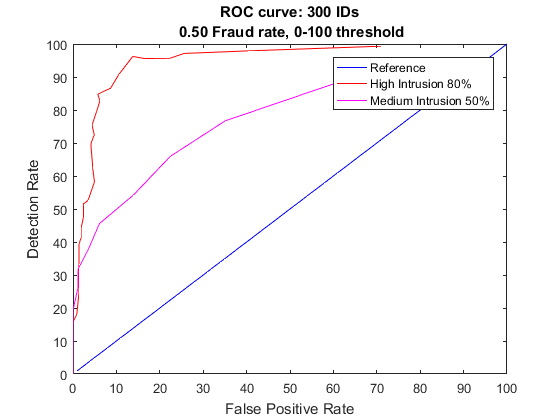
\includegraphics[width=140mm, height=100mm]{../../plots/ROC50_1.png}
\caption{Καμπύλη ROC για FR=0.50 \label{ROC50}}

\begin{center}
\begin{tabu} to 0.8\textwidth { | X[c] | X[c] | X[c] | X[c] | X[c] |  }
 \hline
 \multicolumn{5}{|c|}{300 IDs, 0.5 rate, 0-100 threshold} \\
 \hline
 Όριο (Μέρες)    & DR (0.8) & FPR (0.8) & DR (0.5) & FPR (0.5) \\
 \hline
2 &	 97,917 &	40,385 &	76,712 &	35,0649\\
4 &	 97,143 &	25,625 & 	65,972 &	22,436\\
6 &	 95,683 &	22,360 &	54,225 &	13,924\\
8 &	 95,588 &	16,463 &	45,588 &	6,098\\
10 & 96,241 &	13,772 &	37,879 &	3,571\\
12 & 90,698 &	10,526 &	31,783 &	1,17\\
14 & 86,614 &	8,671  &	26,190 &	1,149\\
16 & 84,8	&	5,714  &	19,355 &	0\\
18 & 82,787 &	6,18   &	15,702 &	0\\
20 & 79,832 &	5,525  &	11,667 &	0\\
\hline
\end{tabu}
\end{center}
\caption{Πίνακας επιλογής ορίου FR=0.5 \label{ROC50data}}
\end{figure}



\begin{figure}[ht!]
\centering
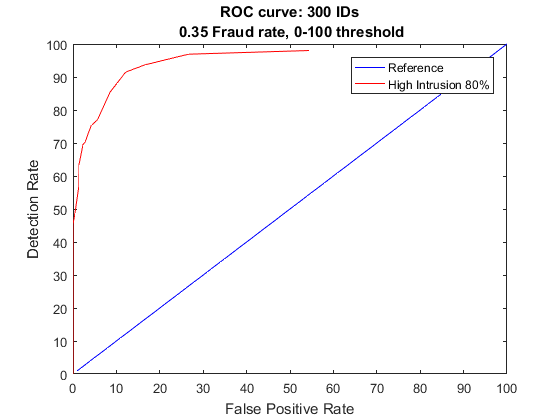
\includegraphics[width=140mm, height=100mm]{../../plots/ROC35.png}
\caption{Καμπύλη ROC για FR=0.35 \label{ROC35}}


\begin{center}
\begin{tabu} to 0.6\textwidth { | X[c] | X[c] | X[c] |  }
 \hline
 \multicolumn{3}{|c|}{300 IDs, 0.35 rate, 0-100 threshold} \\
 \hline
 Όριο (Μέρες)   & DR (0.8) & FPR (0.8)\\
 \hline
2 &	 95,192 &	30,612\\
4 &	 91,176 &	23,232\\
6 &	 89,691 &	17,734\\
8 &	 85,567 &	12,808\\
10 & 85,106 &	8,738\\
12 & 84,444 &	5,238\\
14 & 79,545 &	2,830\\
16 & 75		&	2,830\\
18 & 68,235 &	2,791\\
20 & 63,529 &	2,791\\
\hline
\end{tabu}
\end{center}
\caption{Πίνακας επιλογής ορίου FR=0.35 \label{ROC35data}}
\end{figure}

\newpage
\section*{Συμπεράσματα}
Όπως γίνεται αντιληπτό ο ταξινομητής μας έχει εκπαιδευτεί μόνο για έντονες ρευματοκλοπές που βρίσκονται στο εύρος 0.6-0.9 έντασης κλοπής πράγμα που καθιστά αδύνατη την αναγνώριση επίθεσης στα δεδομένα με χαμηλή ένταση. Παράλληλα, απαιτεί μεγαλύτερος όγκος δεδομένων για να μπορέσει να γίνεται αντιληπτό το πλήθος των παραβατών, όταν το ποσοστό τους είναι μικρό (FΡ<0.35). Τέλος, παρατηρείται πως όσο μικραίνει το ποσοστό απάτης FR το όριο τείνει να μειωθεί, αφού δεν είναι τόσο συχνά τα φαινόνενα απάτης αυξάνεται η ευαισθησία του συστήματος. 

\section*{Συνημμένα}
\ifx
Lab Notes, HelloWorld.ic, FooBar.ic
\fi %comment me out
\ref{type1}.Απώλειες Τύπου 1, \ref{type2}.Απώλειες Τύπου 2, \ref{type3}.Απώλειες Τύπου 3, \ref{type4}.Απώλειες Τύπου 4, \ref{confMatrix}.Πίνακας Λάθους, \ref{ROC50}.Καμπύλη ROC για FR=0.50, \ref{ROC50data}.Πίνακας επιλογής ορίου FR=0.5, \ref{ROC35}.Καμπύλη ROC για FR=0.35, \ref{ROC35data}.Πίνακας επιλογής ορίου FR=0.35


\begin{thebibliography}{9}
\bibitem{NeuralNet} V. Ford, A. Siraj, W. Eberle, 2014. \emph{Smart Grid Energy Fraud Detection Using Artificial Neural Networks}. p. 2.

\bibitem{giwrgis} G. Messinis,  A. Dimeas, 2016. \emph{Utilizing smart meter data for electricity fraud detection}. p. 7.

\bibitem{patterns} P. Jokar, N. Arianpoo, V. C. M. Leung, 2016. \emph{Electricity Theft Detection in AMI Using Customers' Consumption Patterns}. p. 7.

\bibitem{guide} C.-W. Hsu, C.-C. Chang, C.-J. Lin, 2003. \emph{A practical guide to support vector classification }. Technical report, Department of Computer Science, National Taiwan University. July, p. 4,5,14.

\bibitem{propab} S. Axelsson, 1999. \emph{The Base-Rate Fallacy and its Implications for the
Difficulty of Intrusion Detection}. Technical report, Department of Computer Science, Chalmers University of Technology. 20 May, p. 5.

\ifx
\bibitem{Flueck}  Flueck, Alexander J. 2005. \emph{ECE 100}[online]. Chicago: Illinois Institute of Technology, Electrical and Computer Engineering Department, 2005 [cited 30
August 2005]. Available from World Wide Web: (http://www.ece.iit.edu/~flueck/ece100).
\fi
\end{thebibliography}

\end{document}
